\PassOptionsToPackage{unicode=true}{hyperref} % options for packages loaded elsewhere
\PassOptionsToPackage{hyphens}{url}
%
\documentclass[]{article}
\usepackage{lmodern}
\usepackage{amssymb,amsmath}
\usepackage{ifxetex,ifluatex}
\usepackage{fixltx2e} % provides \textsubscript
\ifnum 0\ifxetex 1\fi\ifluatex 1\fi=0 % if pdftex
  \usepackage[T1]{fontenc}
  \usepackage[utf8]{inputenc}
  \usepackage{textcomp} % provides euro and other symbols
\else % if luatex or xelatex
  \usepackage{unicode-math}
  \defaultfontfeatures{Ligatures=TeX,Scale=MatchLowercase}
\fi
% use upquote if available, for straight quotes in verbatim environments
\IfFileExists{upquote.sty}{\usepackage{upquote}}{}
% use microtype if available
\IfFileExists{microtype.sty}{%
\usepackage[]{microtype}
\UseMicrotypeSet[protrusion]{basicmath} % disable protrusion for tt fonts
}{}
\IfFileExists{parskip.sty}{%
\usepackage{parskip}
}{% else
\setlength{\parindent}{0pt}
\setlength{\parskip}{6pt plus 2pt minus 1pt}
}
\usepackage{hyperref}
\hypersetup{
            pdftitle={melbourne\_house\_price\_prediction},
            pdfauthor={Kevin},
            pdfborder={0 0 0},
            breaklinks=true}
\urlstyle{same}  % don't use monospace font for urls
\usepackage[margin=1in]{geometry}
\usepackage{color}
\usepackage{fancyvrb}
\newcommand{\VerbBar}{|}
\newcommand{\VERB}{\Verb[commandchars=\\\{\}]}
\DefineVerbatimEnvironment{Highlighting}{Verbatim}{commandchars=\\\{\}}
% Add ',fontsize=\small' for more characters per line
\usepackage{framed}
\definecolor{shadecolor}{RGB}{248,248,248}
\newenvironment{Shaded}{\begin{snugshade}}{\end{snugshade}}
\newcommand{\AlertTok}[1]{\textcolor[rgb]{0.94,0.16,0.16}{#1}}
\newcommand{\AnnotationTok}[1]{\textcolor[rgb]{0.56,0.35,0.01}{\textbf{\textit{#1}}}}
\newcommand{\AttributeTok}[1]{\textcolor[rgb]{0.77,0.63,0.00}{#1}}
\newcommand{\BaseNTok}[1]{\textcolor[rgb]{0.00,0.00,0.81}{#1}}
\newcommand{\BuiltInTok}[1]{#1}
\newcommand{\CharTok}[1]{\textcolor[rgb]{0.31,0.60,0.02}{#1}}
\newcommand{\CommentTok}[1]{\textcolor[rgb]{0.56,0.35,0.01}{\textit{#1}}}
\newcommand{\CommentVarTok}[1]{\textcolor[rgb]{0.56,0.35,0.01}{\textbf{\textit{#1}}}}
\newcommand{\ConstantTok}[1]{\textcolor[rgb]{0.00,0.00,0.00}{#1}}
\newcommand{\ControlFlowTok}[1]{\textcolor[rgb]{0.13,0.29,0.53}{\textbf{#1}}}
\newcommand{\DataTypeTok}[1]{\textcolor[rgb]{0.13,0.29,0.53}{#1}}
\newcommand{\DecValTok}[1]{\textcolor[rgb]{0.00,0.00,0.81}{#1}}
\newcommand{\DocumentationTok}[1]{\textcolor[rgb]{0.56,0.35,0.01}{\textbf{\textit{#1}}}}
\newcommand{\ErrorTok}[1]{\textcolor[rgb]{0.64,0.00,0.00}{\textbf{#1}}}
\newcommand{\ExtensionTok}[1]{#1}
\newcommand{\FloatTok}[1]{\textcolor[rgb]{0.00,0.00,0.81}{#1}}
\newcommand{\FunctionTok}[1]{\textcolor[rgb]{0.00,0.00,0.00}{#1}}
\newcommand{\ImportTok}[1]{#1}
\newcommand{\InformationTok}[1]{\textcolor[rgb]{0.56,0.35,0.01}{\textbf{\textit{#1}}}}
\newcommand{\KeywordTok}[1]{\textcolor[rgb]{0.13,0.29,0.53}{\textbf{#1}}}
\newcommand{\NormalTok}[1]{#1}
\newcommand{\OperatorTok}[1]{\textcolor[rgb]{0.81,0.36,0.00}{\textbf{#1}}}
\newcommand{\OtherTok}[1]{\textcolor[rgb]{0.56,0.35,0.01}{#1}}
\newcommand{\PreprocessorTok}[1]{\textcolor[rgb]{0.56,0.35,0.01}{\textit{#1}}}
\newcommand{\RegionMarkerTok}[1]{#1}
\newcommand{\SpecialCharTok}[1]{\textcolor[rgb]{0.00,0.00,0.00}{#1}}
\newcommand{\SpecialStringTok}[1]{\textcolor[rgb]{0.31,0.60,0.02}{#1}}
\newcommand{\StringTok}[1]{\textcolor[rgb]{0.31,0.60,0.02}{#1}}
\newcommand{\VariableTok}[1]{\textcolor[rgb]{0.00,0.00,0.00}{#1}}
\newcommand{\VerbatimStringTok}[1]{\textcolor[rgb]{0.31,0.60,0.02}{#1}}
\newcommand{\WarningTok}[1]{\textcolor[rgb]{0.56,0.35,0.01}{\textbf{\textit{#1}}}}
\usepackage{graphicx,grffile}
\makeatletter
\def\maxwidth{\ifdim\Gin@nat@width>\linewidth\linewidth\else\Gin@nat@width\fi}
\def\maxheight{\ifdim\Gin@nat@height>\textheight\textheight\else\Gin@nat@height\fi}
\makeatother
% Scale images if necessary, so that they will not overflow the page
% margins by default, and it is still possible to overwrite the defaults
% using explicit options in \includegraphics[width, height, ...]{}
\setkeys{Gin}{width=\maxwidth,height=\maxheight,keepaspectratio}
\setlength{\emergencystretch}{3em}  % prevent overfull lines
\providecommand{\tightlist}{%
  \setlength{\itemsep}{0pt}\setlength{\parskip}{0pt}}
\setcounter{secnumdepth}{0}
% Redefines (sub)paragraphs to behave more like sections
\ifx\paragraph\undefined\else
\let\oldparagraph\paragraph
\renewcommand{\paragraph}[1]{\oldparagraph{#1}\mbox{}}
\fi
\ifx\subparagraph\undefined\else
\let\oldsubparagraph\subparagraph
\renewcommand{\subparagraph}[1]{\oldsubparagraph{#1}\mbox{}}
\fi

% set default figure placement to htbp
\makeatletter
\def\fps@figure{htbp}
\makeatother


\title{melbourne\_house\_price\_prediction}
\author{Kevin}
\date{29 May 2021}

\begin{document}
\maketitle

\begin{Shaded}
\begin{Highlighting}[]
\KeywordTok{library}\NormalTok{(tidyverse)}
\end{Highlighting}
\end{Shaded}

\begin{verbatim}
## -- Attaching packages --------------------------------------- tidyverse 1.3.1 --
\end{verbatim}

\begin{verbatim}
## v ggplot2 3.3.3     v purrr   0.3.4
## v tibble  3.1.1     v dplyr   1.0.6
## v tidyr   1.1.3     v stringr 1.4.0
## v readr   1.4.0     v forcats 0.5.1
\end{verbatim}

\begin{verbatim}
## -- Conflicts ------------------------------------------ tidyverse_conflicts() --
## x dplyr::filter() masks stats::filter()
## x dplyr::lag()    masks stats::lag()
\end{verbatim}

\begin{Shaded}
\begin{Highlighting}[]
\KeywordTok{library}\NormalTok{(data.table)}
\end{Highlighting}
\end{Shaded}

\begin{verbatim}
## 
## Attaching package: 'data.table'
\end{verbatim}

\begin{verbatim}
## The following objects are masked from 'package:dplyr':
## 
##     between, first, last
\end{verbatim}

\begin{verbatim}
## The following object is masked from 'package:purrr':
## 
##     transpose
\end{verbatim}

\begin{Shaded}
\begin{Highlighting}[]
\NormalTok{house_raw <-}\StringTok{ }\KeywordTok{fread}\NormalTok{(}\StringTok{'data/melb_data.csv'}\NormalTok{, }\DataTypeTok{colClasses =} \KeywordTok{c}\NormalTok{(}\StringTok{'Suburb'}\NormalTok{ =}\StringTok{ 'factor'}\NormalTok{, }\StringTok{'Type'}\NormalTok{ =}\StringTok{ 'factor'}\NormalTok{, }\StringTok{'CouncilArea'}\NormalTok{ =}\StringTok{ 'factor'}\NormalTok{,}
                                                        \StringTok{'Method'}\NormalTok{ =}\StringTok{ 'factor'}\NormalTok{, }\StringTok{'Regionname'}\NormalTok{ =}\StringTok{ 'factor'}\NormalTok{, }\StringTok{'Postcode'}\NormalTok{=}\StringTok{'factor'}\NormalTok{))}
\KeywordTok{summary}\NormalTok{(house_raw)}
\end{Highlighting}
\end{Shaded}

\begin{verbatim}
##             Suburb        Address              Rooms        Type    
##  Reservoir     :  359   Length:13580       Min.   : 1.000   h:9449  
##  Richmond      :  260   Class :character   1st Qu.: 2.000   t:1114  
##  Bentleigh East:  249   Mode  :character   Median : 3.000   u:3017  
##  Preston       :  239                      Mean   : 2.938           
##  Brunswick     :  222                      3rd Qu.: 3.000           
##  Essendon      :  220                      Max.   :10.000           
##  (Other)       :12031                                               
##      Price         Method      SellerG              Date          
##  Min.   :  85000   PI:1564   Length:13580       Length:13580      
##  1st Qu.: 650000   S :9022   Class :character   Class :character  
##  Median : 903000   SA:  92   Mode  :character   Mode  :character  
##  Mean   :1075684   SP:1703                                        
##  3rd Qu.:1330000   VB:1199                                        
##  Max.   :9000000                                                  
##                                                                   
##     Distance        Postcode        Bedroom2         Bathroom    
##  Min.   : 0.00   3073.0 :  359   Min.   : 0.000   Min.   :0.000  
##  1st Qu.: 6.10   3020.0 :  306   1st Qu.: 2.000   1st Qu.:1.000  
##  Median : 9.20   3121.0 :  292   Median : 3.000   Median :1.000  
##  Mean   :10.14   3040.0 :  290   Mean   : 2.915   Mean   :1.534  
##  3rd Qu.:13.00   3046.0 :  284   3rd Qu.: 3.000   3rd Qu.:2.000  
##  Max.   :48.10   3165.0 :  249   Max.   :20.000   Max.   :8.000  
##                  (Other):11800                                   
##       Car           Landsize         BuildingArea     YearBuilt   
##  Min.   : 0.00   Min.   :     0.0   Min.   :    0   Min.   :1196  
##  1st Qu.: 1.00   1st Qu.:   177.0   1st Qu.:   93   1st Qu.:1940  
##  Median : 2.00   Median :   440.0   Median :  126   Median :1970  
##  Mean   : 1.61   Mean   :   558.4   Mean   :  152   Mean   :1965  
##  3rd Qu.: 2.00   3rd Qu.:   651.0   3rd Qu.:  174   3rd Qu.:1999  
##  Max.   :10.00   Max.   :433014.0   Max.   :44515   Max.   :2018  
##  NA's   :62                         NA's   :6450    NA's   :5375  
##         CouncilArea     Lattitude        Longtitude   
##               :1369   Min.   :-38.18   Min.   :144.4  
##  Moreland     :1163   1st Qu.:-37.86   1st Qu.:144.9  
##  Boroondara   :1160   Median :-37.80   Median :145.0  
##  Moonee Valley: 997   Mean   :-37.81   Mean   :145.0  
##  Darebin      : 934   3rd Qu.:-37.76   3rd Qu.:145.1  
##  Glen Eira    : 848   Max.   :-37.41   Max.   :145.5  
##  (Other)      :7109                                   
##                       Regionname   Propertycount  
##  Southern Metropolitan     :4695   Min.   :  249  
##  Northern Metropolitan     :3890   1st Qu.: 4380  
##  Western Metropolitan      :2948   Median : 6555  
##  Eastern Metropolitan      :1471   Mean   : 7454  
##  South-Eastern Metropolitan: 450   3rd Qu.:10331  
##  Eastern Victoria          :  53   Max.   :21650  
##  (Other)                   :  73
\end{verbatim}

\hypertarget{missing-data-imputationmean}{%
\subsection{Missing Data
Imputation(Mean)}\label{missing-data-imputationmean}}

\begin{Shaded}
\begin{Highlighting}[]
\NormalTok{house_raw <-}\StringTok{ }\NormalTok{house_raw }\OperatorTok\StringTok{ }\KeywordTok{mutate_at}\NormalTok{(}\KeywordTok{vars}\NormalTok{(Car),}\OperatorTok{~}\KeywordTok{ifelse}\NormalTok{(}\KeywordTok{is.na}\NormalTok{(.x), }\KeywordTok{mean}\NormalTok{(.x, }\DataTypeTok{na.rm =} \OtherTok{TRUE}\NormalTok{), .x))}
\end{Highlighting}
\end{Shaded}

\begin{Shaded}
\begin{Highlighting}[]
\KeywordTok{set.seed}\NormalTok{(}\DecValTok{101}\NormalTok{) }
\NormalTok{sample <-}\StringTok{ }\KeywordTok{sample.int}\NormalTok{(}\DataTypeTok{n =} \KeywordTok{nrow}\NormalTok{(house_raw), }\DataTypeTok{size =} \KeywordTok{floor}\NormalTok{(.}\DecValTok{8}\OperatorTok{*}\KeywordTok{nrow}\NormalTok{(house_raw)), }\DataTypeTok{replace =}\NormalTok{ F)}
\NormalTok{train <-}\StringTok{ }\NormalTok{house_raw[sample, ]}
\NormalTok{test  <-}\StringTok{ }\NormalTok{house_raw[}\OperatorTok{-}\NormalTok{sample, ]}
\end{Highlighting}
\end{Shaded}

\hypertarget{baseline---only-numeric-featuresrooms-distance-bedroom2-bathroom-car-landsize-lattitude-longitude-propertycount}{%
\subsection{Baseline - Only numeric features(Rooms, Distance, Bedroom2,
Bathroom, Car, Landsize, Lattitude, Longitude,
Propertycount)}\label{baseline---only-numeric-featuresrooms-distance-bedroom2-bathroom-car-landsize-lattitude-longitude-propertycount}}

(Ignoring BuildingArea and YearBuilt)

\begin{Shaded}
\begin{Highlighting}[]
\NormalTok{RMSE <-}\StringTok{ }\ControlFlowTok{function}\NormalTok{(error) \{ }\KeywordTok{sqrt}\NormalTok{(}\KeywordTok{mean}\NormalTok{(error}\OperatorTok{^}\DecValTok{2}\NormalTok{)) \}}
\NormalTok{base_model <-}\StringTok{ }\KeywordTok{lm}\NormalTok{(Price }\OperatorTok{~}\StringTok{ }\NormalTok{Rooms }\OperatorTok{+}\StringTok{ }\NormalTok{Distance }\OperatorTok{+}\StringTok{ }\NormalTok{Bedroom2 }\OperatorTok{+}\StringTok{ }\NormalTok{Bathroom }\OperatorTok{+}\StringTok{ }\NormalTok{Car }\OperatorTok{+}\StringTok{ }\NormalTok{Landsize }\OperatorTok{+}
\StringTok{              }\NormalTok{Lattitude }\OperatorTok{+}\StringTok{ }\NormalTok{Longtitude }\OperatorTok{+}\StringTok{ }\NormalTok{Propertycount, }\DataTypeTok{data=}\NormalTok{train)}
\KeywordTok{summary}\NormalTok{(base_model)}
\end{Highlighting}
\end{Shaded}

\begin{verbatim}
## 
## Call:
## lm(formula = Price ~ Rooms + Distance + Bedroom2 + Bathroom + 
##     Car + Landsize + Lattitude + Longtitude + Propertycount, 
##     data = train)
## 
## Residuals:
##      Min       1Q   Median       3Q      Max 
## -2442759  -275568   -68319   179306  8045151 
## 
## Coefficients:
##                 Estimate Std. Error t value Pr(>|t|)    
## (Intercept)   -2.020e+08  6.554e+06 -30.825  < 2e-16 ***
## Rooms          2.318e+05  1.630e+04  14.221  < 2e-16 ***
## Distance      -4.478e+04  8.415e+02 -53.216  < 2e-16 ***
## Bedroom2       7.865e+04  1.635e+04   4.810 1.53e-06 ***
## Bathroom       1.740e+05  8.260e+03  21.068  < 2e-16 ***
## Car            5.953e+04  5.289e+03  11.255  < 2e-16 ***
## Landsize       1.666e+01  2.883e+00   5.778 7.77e-09 ***
## Lattitude     -1.703e+06  6.123e+04 -27.823  < 2e-16 ***
## Longtitude     9.511e+05  4.801e+04  19.809  < 2e-16 ***
## Propertycount -2.513e+00  1.030e+00  -2.439   0.0147 *  
## ---
## Signif. codes:  0 '***' 0.001 '**' 0.01 '*' 0.05 '.' 0.1 ' ' 1
## 
## Residual standard error: 468500 on 10854 degrees of freedom
## Multiple R-squared:  0.4807, Adjusted R-squared:  0.4803 
## F-statistic:  1116 on 9 and 10854 DF,  p-value: < 2.2e-16
\end{verbatim}

\begin{Shaded}
\begin{Highlighting}[]
\KeywordTok{RMSE}\NormalTok{(base_model}\OperatorTok{$}\NormalTok{residuals)}
\end{Highlighting}
\end{Shaded}

\begin{verbatim}
## [1] 468309.9
\end{verbatim}

\begin{Shaded}
\begin{Highlighting}[]
\KeywordTok{plot}\NormalTok{(}\DataTypeTok{x=}\NormalTok{base_model}\OperatorTok{$}\NormalTok{fitted.values, }\DataTypeTok{y=}\NormalTok{base_model}\OperatorTok{$}\NormalTok{residuals)}
\end{Highlighting}
\end{Shaded}

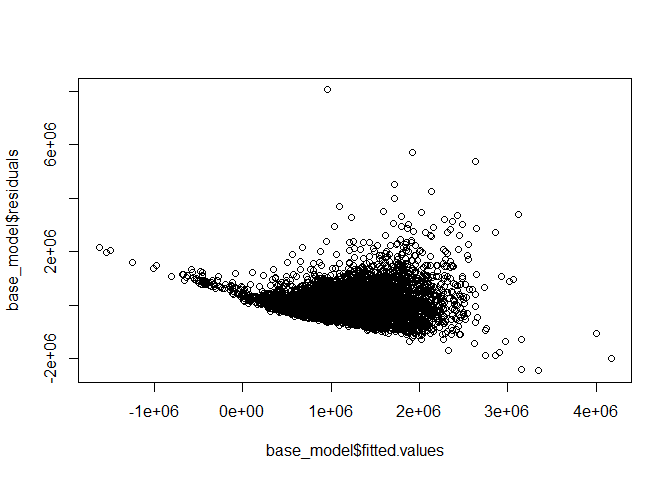
\includegraphics{melborne_price_prediction_files/figure-latex/unnamed-chunk-6-1.pdf}

\end{document}
